\begin{frame}{The Fixed Point Theorem}
  \begin{columns}[c]
    \begin{column}{0.8\textwidth}
      \begin{itemize}
      \item In a Lattice L
      \item Every monotone function $f$ has a unique least fixed-point:
      \end{itemize}
      \[ fix(f) = \bigsqcup_{i \ge 0} f^i(\bot) \]
    \end{column}
    
    \begin{column}{0.2\textwidth}
      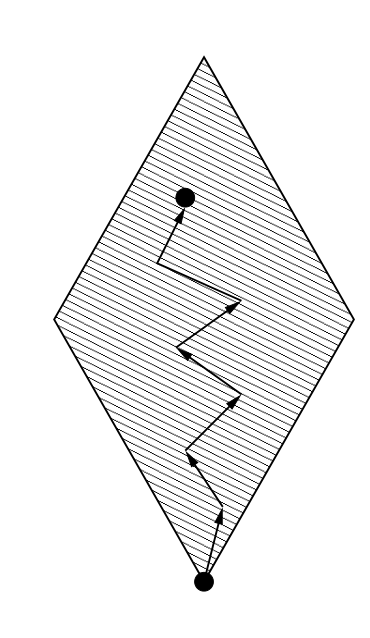
\includegraphics[width=\textwidth]{graphics/fixed-point_walk}
    \end{column}
  \end{columns}
\end{frame}

\begin{frame}{The Fixed Point Theorem}
  \begin{columns}[c]
    \begin{column}{0.8\textwidth}
      \noindent
      \[
      \begin{array}{l}
        \only<1>{\bot \sqsubseteq f(\bot) \phantom{\bot \sqsubseteq \dots}\\
        \phantom{}\\}
        \only<2->{\bot \sqsubseteq f(\bot) \sqsubseteq f^2(\bot) \sqsubseteq \dots\\
        \phantom{}\\}
        \onslide<3->{\dots \sqsubseteq f^k(\bot) \sqsubseteq f^{k+1}(\bot)\\
        \phantom{}\\}
        \onslide<4->{f^k(\bot) = fix(f)}
      \end{array}
      \]
    \end{column}

    \begin{column}<0->{0.2\textwidth}
      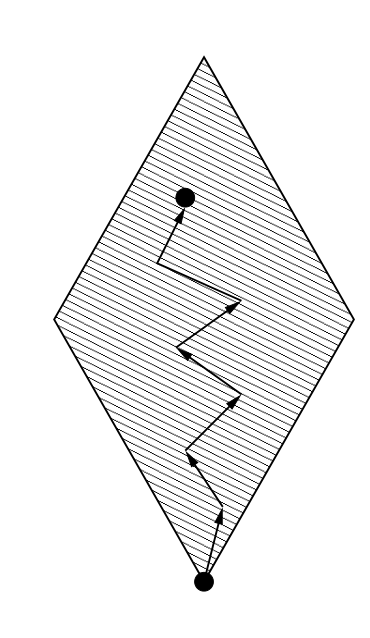
\includegraphics[width=\textwidth]{graphics/fixed-point_walk}
    \end{column}
  \end{columns}
\end{frame}


\begin{frame}{Constraint Rules}{}
  Our f is defined by a number of constraint rules, applied on each CFG node, yielding the function:
  \[ F(x_1, \dots, x_n) = (F_1(x_1, \dots, x_n), \dots, F_n(x_1, \dots, x_n)) \]

  (CFG udsnit med F\_1, F\_2 omkring nodes)
\end{frame}


\begin{frame}{Constraint Rules}{}
  {\color{red} Forward} analysis:
  \[ JOIN(v) = \bigcup_{ w \in pred(v)} \constraint{w} \]

  Non-assignment nodes:
    \[ \constraint{v} = JOIN(v) \]
\end{frame}


\begin{frame}{Constraint Rules}{}
    Assignment nodes:
  \begin{align*}
  \constraint{v} = &\text{ if v is a reassignment:}\\
  &\phantom{==}JOIN(v) \cup \{ v \}\\
  &\text{ else:}\\
  &\phantom{==}JOIN(v) \downarrow id \cup \{ v \}\\
  \end{align*}
\end{frame}

\begin{frame}
\[
\begin{array}{lclcl}
  \constraint{entry} & = & \{\} &\phantom{hahahahhh}\\
  \assignconstraint{param} & = & \{\} &\\
  \assignconstraint{command} & = & \{\}&\\
  \constraint{subprocess.call} & = & \{\}&\\
  \constraint{with} & = & \{\}&\\
  \assignconstraint{menu} & = & \{\}&\\
  \assignconstraint{ret\_f.read} & = & \{\}&\\
  \constraint{exit} & = & \{\}&\\
  && \phantom{\{command, param\}} && \phantom{\{command, param\}}
\end{array}
\]
\end{frame}

\begin{frame}
\[
\begin{array}{lclcl}
  \constraint{entry} & = & \{\} & \rightarrow & \{\}\\
  \assignconstraint{param} & = & \{\} & \rightarrow &\{param\}\\
  \assignconstraint{command} & = & \{\}& \rightarrow &\{command\}\\
  \constraint{subprocess.call} & = & \{\}& \rightarrow &\{\}\\
  \constraint{with} & = & \{\}&\rightarrow & \{\}\\
  \assignconstraint{menu} & = & \{\}& \rightarrow & \{menu\}\\
  \assignconstraint{ret\_f.read} & = & \{\}&\rightarrow & \{ret\_f.read\}\\
  \constraint{exit} & = & \{\}&\rightarrow & \{\}\\
  && && \phantom{\{command, param\}\{command, param\}}
\end{array}
\]
\end{frame}

\begin{frame}
\[
\begin{array}{lclcl}
  \constraint{entry} & = &  \{\} & \phantom{\rightarrow} & \phantom{hahahaha}\\
  \assignconstraint{param} & = & \{param\}&  & \\ 
  \assignconstraint{command} & = &\{command\}&  & \\
  \constraint{subprocess.call} & = & \{\}&  & \\
  \constraint{with} & = & \{\}&  & \\
  \assignconstraint{menu} & = &  \{menu\}&  & \\
  \assignconstraint{ret\_f.read} & = & \{ret\_f.read\}&  & \\
  \constraint{exit} & = & \{\}&  & \\
  && && \phantom{\{command, param\} \{command, param\}}
\end{array}
\]
\end{frame}

\begin{frame}
  \[
\begin{array}{lclcl}
  \constraint{entry} & = &  \{\} & \rightarrow & \{\}\\
  \assignconstraint{param} & = & \{param\}& \rightarrow & \{param\}\\ 
  \assignconstraint{command} & = &\{command\}& \rightarrow & \{command, param\}\\
  \constraint{subprocess.call} & = & \{\}& \rightarrow & \{command\}\\
  \constraint{with} & = & \{\}& \rightarrow & \{\}\\
  \assignconstraint{menu} & = &  \{menu \}& \rightarrow & \{menu\} \\
  \assignconstraint{ret\_f.read} & = & \{ret\_f.read\}& \rightarrow & \{ret\_f.read, menu\}\\
  \constraint{exit} & = & \{\}& \rightarrow & \{ret\_f.read\}\\
  && && \phantom{\{command, param\}\{command, param\}}
\end{array}
\]
\end{frame}


\begin{frame}
  \[
\begin{array}{lclcl}
  \constraint{entry} & = & \{\}& \phantom{\rightarrow} & \phantom{\{command, param\}} \\
  \assignconstraint{param} & = & \{param\}& \\ 
  \assignconstraint{command} & = & \{command, param\}& \\
  \constraint{subprocess.call} & = & \{command\}& \\
  \constraint{with} & = & \{\}& \\
  \assignconstraint{menu} & = & \{menu\} & \\
  \assignconstraint{ret\_f.read} & = & \{ret\_f.read, menu\}& \\
  \constraint{exit} & = & \{ret\_f.read\}& \\
  && \phantom{\{command, param\}} && \phantom{\{command, param\}}
\end{array}
\]
\end{frame}


\begin{frame}
  \[
\begin{array}{lclcl}
  \constraint{entry} & = & \{\}& \rightarrow & \{\} \\
  \assignconstraint{param} & = & \{param\}& \rightarrow & \{param\}\\ 
  \assignconstraint{command} & = & \{command , param \}& \rightarrow & \{command, param\}\\
  \constraint{subprocess.call} & = & \{command\}& \rightarrow & \{command, param\}\\
  \constraint{with} & = & \{\}& \rightarrow & \{command\}\\
  \assignconstraint{menu} & = & \{menu\} & \rightarrow & \{menu\}\\
  \assignconstraint{ret\_f.read} & = & \{ret\_f.read, menu\}& \rightarrow & \{ret_f.read, menu\}\\
  \constraint{exit} & = & \{ret\_f.read\}& \rightarrow & \{ret_f.read, menu\}\\
  && && \phantom{\{command, param\}}
\end{array}
\]
\end{frame}

\begin{frame}
  \[
\begin{array}{lclcl}
  \constraint{entry} & = & \{command, param\} & \phantom{\rightarrow} & \phantom{\{command, param\}}\\
  \assignconstraint{param} & = & \{param\} \\ 
  \assignconstraint{command} & = & \{command, param\}\\
  \constraint{subprocess.call} & = & \{command, param\}\\
  \constraint{with} & = & \{command\} \\
  \assignconstraint{menu} & = & \{menu\}\\
  \assignconstraint{ret\_f.read} & = & \{ret_f.read, menu\}\\
  \constraint{exit} & = & \{ret_f.read, menu\}\\
  &&  && \phantom{\{command, param\}}
\end{array}
\]
\end{frame}

\begin{frame}
  \[
\begin{array}{lclcl}
  \constraint{entry} & = & \dots & \rightarrow & {\{\}}\\
  \assignconstraint{param} & = & \dots & \rightarrow & \{param\} \\ 
  \assignconstraint{command} & = & \dots & \rightarrow & \{command, param\}\\
  \constraint{subprocess.call} & = & \dots & \rightarrow & \{command, param\}\\
  \constraint{with} & = & \dots & \rightarrow & \{command, param\} \\
  \assignconstraint{menu} & = & \dots & \rightarrow & \{menu, command, param\}\\
  \assignconstraint{ret\_f.read} & = & \dots & \rightarrow & \{ret_f.read, menu, command, param\}\\
  \constraint{exit} & = & \dots & \rightarrow & \{ret_f.read, menu, command, param\}\\
  &&&&
\end{array}
\]
\end{frame}

\begin{frame}{Flexible analysis}
  The analysis is flexible
  \begin{itemize}
    \item Can be exchanged
    \item Can be extended
  \end{itemize}

 Extension example:
  \begin{itemize}
    \item Dead code analysis
    \item Har vi andre forslag?
  \end{itemize}
  \center
  
\includegraphics[width=0.3\textwidth]{graphics/modular}
\end{frame}

